\chapter{Resultados}\label{capit:cap5}
\vspace{-2.0325ex}%
\noindent
\rule{\textwidth}{0.5pt}
\vspace{-5.5ex}% 
\newcommand{\pushline}{\Indp}% Indent puede ir o no :p

En este capítulo se presentan los resultados de las pruebas realizadas al sistema. El desempeño del sistema es evaluado con respecto a la precisi\'on de la clasificación.   

Los experimentos y el sistema propuesto fue implementado en una computadora de escritorio Dell con un procesador Intel(R) Xeon(R) CPU E5-1603, 16GB de memoria RAM, Windows 7 de 64 bits. La implementación del sistema se realizó en Microsoft C\# utilizando Emgu 2.410 \footnote{\url{http://www.emgu.com/wiki/index.php/Main\_Page}} una adaptacion de OpenCV\footnote{\url{http://opencv.org/}} para C\#. 

Para analizar la tasa de precisión de reconocimiento del sistema propuesto se realizaron varios experimentos en distintas circunstancias. Se analizó el rendimiento del sistema a tres diferentes distancias $70$, $80$, $90$ $cm$ del Kinect frontal. También en diferentes circunstancias de iluminación, con iluminación estándar, media y sin iluminación. Se escogió este tipo de escenarios para evaluar el sistema, para obtener el rendimiento en situaciones que representen o estén en condiciones naturales o reales.

Se utilizaron imágenes reales capturadas por ambos sensores de profundidad del Kinect de $640 \times 480$ pixeles. Las imágenes son cinco personas distintas, realizando los gestos de puño y el de palma de la mano con los dedos separados, para los gestos estáticos. Para los gestos dinámicos se tomaron los gestos de tres personas cada una de ellas realizando los gestos estáticos en movimiento.

Los gestos se realizaron usando una sola mano, en este caso todos los usuarios optaron por usar la mano derecha. Pero el sistema est\'a hecho para que funcione sin importar la mano que se utilice. La mano del usuario tiene que tener una ligera rotación en el eje vertical para que el sistema pueda detectar el gesto.

En cada experimento se analiz\'o el rendimiento del sistema usando un solo dispositivo, el Kinect frontal y usando los dos dispositivos.  


%::::::::::::::::::::::::::::::::::::::::::::::::::::::::::::::::::::::::::::::::::::::::::::::::::::::::::::::::::::::::::


\section{Experimentos de gestos estáticos}\label{TestStaticGestures}  

La evaluación del sistema en cuanto al reconocimiento de los gestos estáticos, se determin\'o conforme al resultado de los experimentos realizados en circunstancias de iluminación, (estándar, media, baja). En cada conjunto de experimentos se tom\'o en cuenta la distancia, ya que en cada grupo se analizaron tres diferentes distancias: $70$, $80$, $90$ $cm$.  

Se analizaron dos gestos estáticos, la palma de la mano con los dedos separados, Gesto 1 y el puño, Gesto 2, de cinco usuarios distintos. Para cada experimento se escogió al azar doscientas imágenes de cada gesto del conjunto de las imágenes capturadas. Cada imagen de un gesto tenia su correspondiente imagen con el Kinect lateral, de manera que eran cuatrocientas imágenes por cada gesto. 

En el análisis del sistema con un solo Kinect, solo se tomaron las imágenes provenientes del Kinect frontal. Para el análisis con dos Kinect se tomaron estas mismas imágenes del Kinect frontal con su correspondiente imagen del Kinect lateral.

Enseguida se presentan los resultados de cada experimento realizado.

%----

\subsection{Experimentos con iluminación} 
Para este experimento se usaron imágenes capturadas en un laboratorio con iluminación estándar, como la que se muestra en la Figura \ref{fig:LabIluminado}. Se tomaron en cuenta tres distancias distintas. 

\begin{figure}[h!]
\begin{center} 
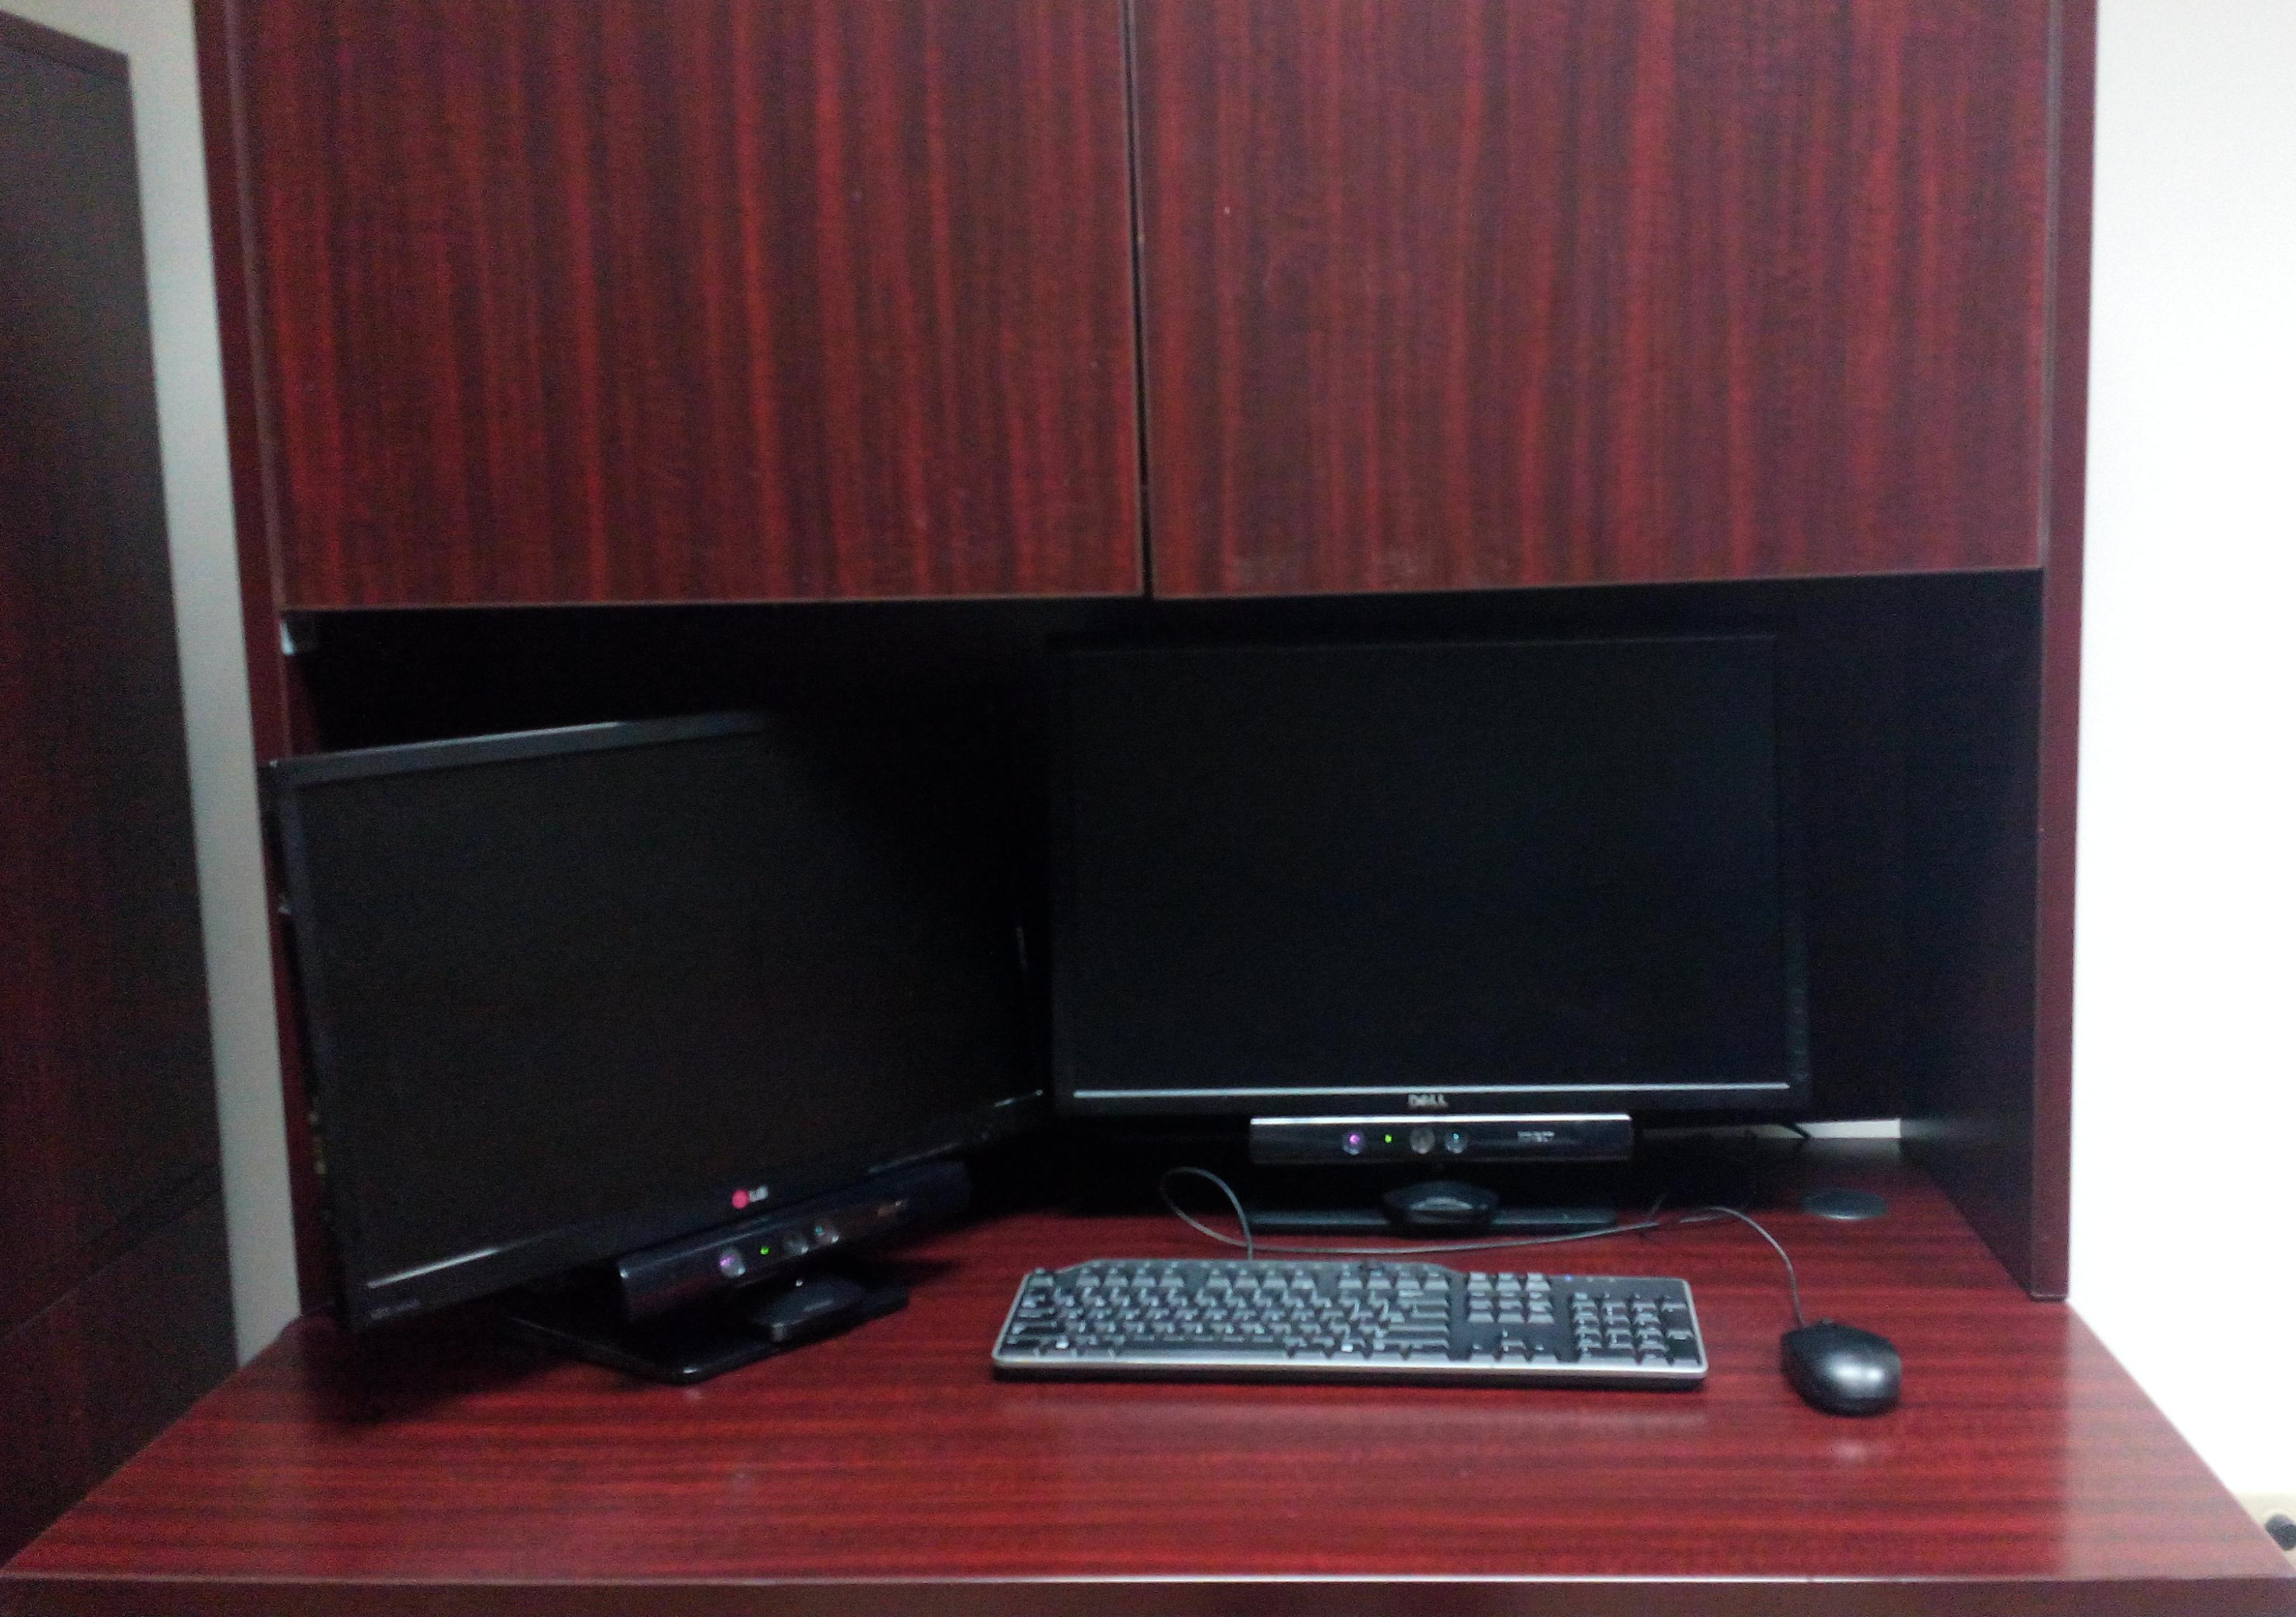
\includegraphics[scale=0.09]{./Figures/iluminacion.jpg}
\end{center}
\caption{Laboratorio en condiciones estándar de iluminación.}
\label{fig:LabIluminado}
\end{figure} 

\begin{itemize}

\item En el primer experimento el usuario se encuentra a una distancia de $70$ $cm$ del Kinect frontal. En la Tabla \ref{table:70L2K} se encuentran los resultados del reconocimiento de los dos gestos utilizando los dos dispositivos y en la Tabla \ref{table:70L1K} los resultados usando un dispositivo.  

%\begin{figure}[h!]
%\centering
%\subfigure[Gesto 1 vista desde el Kinect frontal]{
\includegraphics[scale=.3]{./Figures/pusheen}\label{fig:iluminacion70:1}}
%\subfigure[Gesto 1 viata desde el Kinect lateral]{
\includegraphics[scale=.3]{./Figures/pusheen}\label{fig:iluminacion70:2}}
%\subfigure[Gesto 2 vista desde Kinect frontal]{
\includegraphics[scale=.3]{./Figures/pusheen}\label{fig:iluminacion70:3}}
%\subfigure[Gesto 2 vista desde Kinect lateral]{
\includegraphics[scale=.3]{./Figures/pusheen}\label{fig:iluminacion70:4}}
%\caption{Ejemplo de la imagenes capturadas a una distancia de $70$ $cm$.} \label{fig:iluminacion70}
%\end{figure}

\begin{table}[h!] 
\begin{center} 
\caption{Matriz de confusión del experimento con iluminación estándar, a una distancia de 70 cm utilizando ambos Kinect.} 
\label{table:70L2K} 
\renewcommand{\arraystretch}{1.2}
\begin{tabular}{ r || c  c }  
        & \textbf{Gesto 1} & \textbf{Gesto 2} \\ \hline \hline  
\textbf{Gesto 1} & 170  &  30  \\ \hline  
\textbf{Gesto 2} & 21   & 179 \\   
\end{tabular}
\end{center} 
\end{table}

La matriz de confusión muestra que $170$ gestos de la clase 1 y $179$ de la clase 2 fueron clasificados correctamente. De manera que se obtuvo una tasa de exactitud de $87.25 \%$  

\begin{table}[h!] 
\begin{center}
\caption{Matriz de confusión del experimento con iluminación estándar, a una distancia de 70 cm utilizando el Kinect frontal.}
\label{table:70L1K} 
\renewcommand{\arraystretch}{1.2}
\begin{tabular}{ r || c  c } 
        & \textbf{Gesto 1} & \textbf{Gesto 2} \\ \hline \hline  
\textbf{Gesto 1} & 127  &  73  \\ \hline  
\textbf{Gesto 2} & 6    &  194 \\   
\end{tabular}
\end{center} 
\end{table}

La matriz de confusión muestra que $127$ gestos de la clase 1 y $194$ de la clase 2 fueron clasificados correctamente. De manera que se obtuvo una tasa de exactitud de $80.25\%$. 
 
Como se observa en las matrices de confusión, se obtiene una mayor exactitud en el reconocimiento del gesto utilizando dos dispositivos Kinect.

%----

\item En el segundo experimento el usuario est\'a una distancia de $80$ $cm$ del Kinect frontal. En la Tabla \ref{table:80LK2} se encuentran los resultados del reconocimiento de los dos gestos utilizando los dos dispositivos y en la Tabla \ref{table:80LK1} los resultados usando un dispositivo.   

%\begin{figure}[h!]
%\centering
%\subfigure[Gesto 1 vista desde el Kinect frontal]{
\includegraphics[scale=.3]{./Figures/pusheen}\label{fig:iluminacion80:1}}
%\subfigure[Gesto 1 viata desde el Kinect lateral]{
\includegraphics[scale=.3]{./Figures/pusheen}\label{fig:iluminacion80:2}}
%\subfigure[Gesto 2 vista desde Kinect frontal]{
\includegraphics[scale=.3]{./Figures/pusheen}\label{fig:iluminacion80:3}}
%\subfigure[Gesto 2 vista desde Kinect lateral]{
\includegraphics[scale=.3]{./Figures/pusheen}\label{fig:iluminacion80:4}}
%\caption{Ejemplo de la imagenes capturadas a una distancia de $80$ $cm$.} \label{fig:iluminacion80}
%\end{figure}

\begin{table}[h!] 
\begin{center}
\caption{Matriz de confusión del experimento con iluminación estándar, a una distancia de 80 cm utilizando ambos Kinect.} 
\label{table:80LK2}
\renewcommand{\arraystretch}{1.2}
\begin{tabular}{ r || c  c } 
        & \textbf{Gesto 1} & \textbf{Gesto 2} \\ \hline \hline  
\textbf{Gesto 1} & 96     &  104     \\ \hline  
\textbf{Gesto 2} & 16     & 185     \\   
\end{tabular}
\end{center} 
\end{table}

La matriz de confusión muestra que $96$ gestos de la clase 1 y $185$ de la clase 2 fueron clasificados correctamente. De manera que se obtuvo una tasa de exactitud de $70.25\%$  

\begin{table}[h!] 
\begin{center} 
\caption{Matriz de confusión del experimento con iluminación estándar, a una distancia de 80 cm utilizando el Kinect frontal.} 
\label{table:80LK1}
\renewcommand{\arraystretch}{1.2}
\begin{tabular}{ r || c  c }  
        & \textbf{Gesto 1} & \textbf{Gesto 2} \\ \hline \hline  
\textbf{Gesto 1} & 88     &  112     \\ \hline  
\textbf{Gesto 2} & 6     & 183     \\   
\end{tabular}
\end{center} 
\end{table}  

La matriz de confusión muestra que $88$ gestos de la clase 1 y $183$ de la clase 2 fueron clasificados correctamente. De manera que se obtuvo una tasa de exactitud de $70.5\%$ 

En este experimento la exactitud del reconocimiento es baja para el uso de ambos o un dispositivo Kinect. Se observa, que clasifica los gestos de la clase uno como de la clase dos, esto es debido a la calidad de la imágenes debido a que el sensor no siempre proporciona información detallada o completa de la mano.  


%--- 

\item En el tercer experimento el usuario esta a una distancia de $90$ $cm$ del Kinect frontal. En la Tabla \ref{table:90LK2} se encuentran los resultados del reconocimiento de los dos gestos utilizando los dos dispositivos y en la Tabla \ref{table:90LK1} los resultados usando un dispositivo.   
 
%\begin{figure}[h!]
%\centering
%\subfigure[Gesto 1 vista desde el Kinect frontal]{
\includegraphics[scale=.3]{./Figures/pusheen}\label{fig:iluminacion90:1}}
%\subfigure[\textbf{Gesto 1} viata desde el Kinect lateral]{
\includegraphics[scale=.3]{./Figures/pusheen}\label{fig:iluminacion90:2}}
%\subfigure[Gesto 2 vista desde Kinect frontal]{
\includegraphics[scale=.3]{./Figures/pusheen}\label{fig:iluminacion90:3}}
%\subfigure[Gesto 2 vista desde Kinect lateral]{
\includegraphics[scale=.3]{./Figures/pusheen}\label{fig:iluminacion90:4}}
%\caption{Ejemplo de la imagenes capturadas a una distancia de $90$ $cm$.} \label{fig:iluminacion70}
%\end{figure}

\begin{table}[h!] 
\begin{center}
\caption{Matriz de confusión del experimento con iluminación estándar, a una distancia de 90 cm utilizando ambos Kinect.}
\label{table:90LK2} 
\renewcommand{\arraystretch}{1.2}
\begin{tabular}{ r || c  c } 
        & \textbf{Gesto 1} & \textbf{Gesto 2} \\ \hline \hline  
\textbf{Gesto 1} &  93    & 107      \\ \hline  
\textbf{Gesto 2} &  10    & 190     \\   
\end{tabular}
\end{center} 
\end{table} 

La matriz de confusión muestra que $93$ gestos de la clase 1 y $190$ de la clase 2 fueron clasificados correctamente. De manera que se obtuvo una tasa de exactitud de $70.75\%$ 

\begin{table}[h!] 
\begin{center}
\caption{Matriz de confusión del experimento con iluminación estándar, a una distancia de 90 cm utilizando el Kinect frontal.}
\label{table:90LK1} 
\renewcommand{\arraystretch}{1.2}
\begin{tabular}{ r || c  c } 
        & \textbf{Gesto 1} & \textbf{Gesto 2} \\ \hline \hline  
\textbf{Gesto 1} &  101   & 99      \\ \hline  
\textbf{Gesto 2} &  17    & 183     \\   
\end{tabular}
\end{center} 
\end{table} 

La matriz de confusión muestra que $101$ gestos de la clase 1 y $183$ de la clase 2 fueron clasificados correctamente. De manera que se obtuvo una tasa de exactitud de $71 \%$  

\end{itemize}

En este experimento se observa un resultado similar al anterior, pues otra vez se obtiene baja exactitud en el reconocimiento porque clasifica mal el Gesto 1. Esto por la misma razón del experimento anterior.

%::::::


\subsection{Experimentos con iluminación media} 
Para el conjunto de estos experimentos, las imágenes se capturaron en un laboratorio con iluminación media, como la que se muestra en la Figura \ref{fig:LabMedioIluminado}. A dos distancias $70$ y $90$ $cm$.  

\begin{figure}[h!]
\begin{center} 
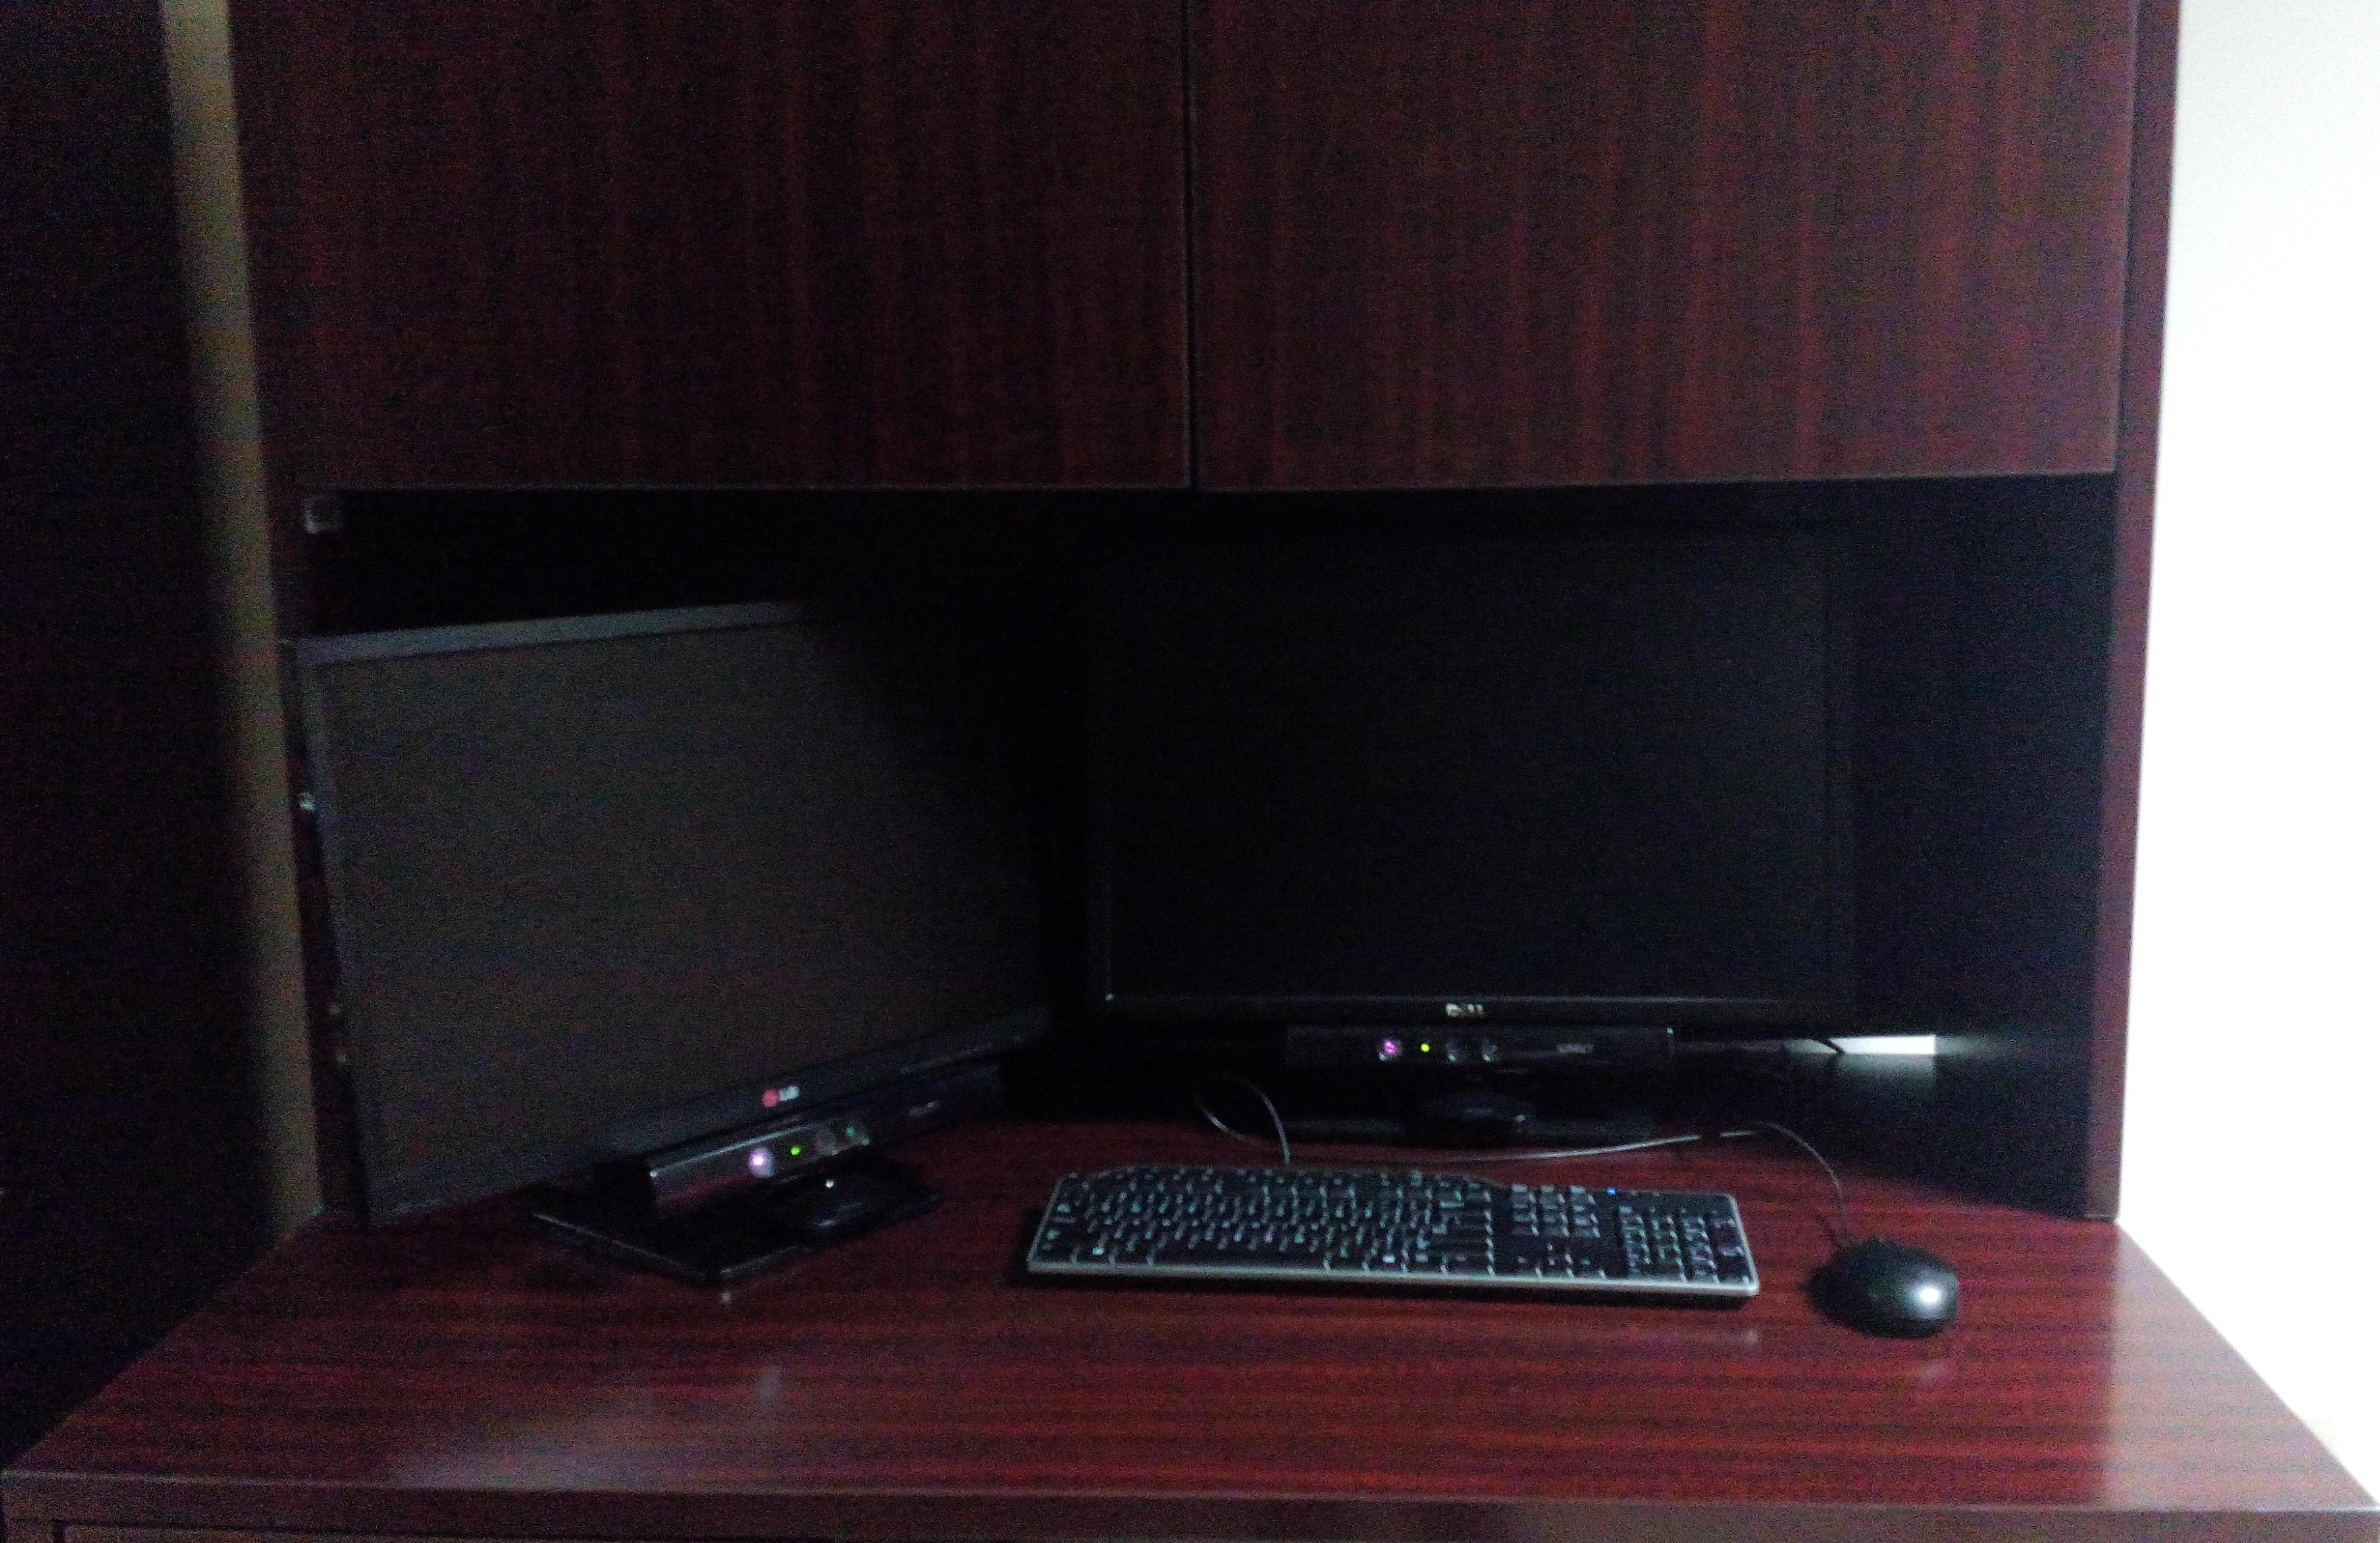
\includegraphics[scale=0.09]{./Figures/mediailuminacion.jpg}
\end{center}
\caption{Laboratorio en condiciones con iluminación media.}
\label{fig:LabMedioIluminado} 
\end{figure}  

%----

\begin{itemize}

\item En el primer experimento el usuario esta a una distancia de $70$ $cm$ del Kinect frontal. En la Tabla \ref{table:70LMK2} se encuentran los resultados del reconocimiento de los dos gestos utilizando los dos dispositivos y en la Tabla \ref{table:70LMK1} los resultados usando un dispositivo.  

%\begin{figure}[h!]
%\centering
%\subfigure[Gesto 1 vista desde el Kinect frontal]{
\includegraphics[scale=.3]{./Figures/pusheen}\label{fig:iluminacionM70:1}}
%\subfigure[Gesto 1 viata desde el Kinect lateral]{
\includegraphics[scale=.3]{./Figures/pusheen}\label{fig:iluminacionM70:2}}
%\subfigure[Gesto 2 vista desde Kinect frontal]{
\includegraphics[scale=.3]{./Figures/pusheen}\label{fig:iluminacionM70:3}}
%\subfigure[Gesto 2 vista desde Kinect lateral]{
\includegraphics[scale=.3]{./Figures/pusheen}\label{fig:iluminacionM70:4}}
%\caption{Ejemplo de la imagenes capturadas a una distancia de $70$ $cm$.} \label{fig:iluminacionM70}
%\end{figure}

\begin{table}[h!] 
\begin{center}
\caption{Matriz de confusión del experimento con iluminación media, a una distancia de 70 cm utilizando ambos Kinect.}
\label{table:70LMK2} 
\renewcommand{\arraystretch}{1.2}
\begin{tabular}{ r || c  c }  
        & \textbf{Gesto 1} & \textbf{Gesto 2} \\ \hline \hline  
\textbf{Gesto 1} & 178    &  22     \\ \hline  
\textbf{Gesto 2} & 84     & 105     \\   
\end{tabular}
\end{center} 

\end{table}

La matriz de confusión muestra que $178$ gestos de la clase 1 y $105$ de la clase 2 fueron clasificados correctamente. De manera que se obtuvo una tasa de exactitud de $72.75 \%$ 

\begin{table}[h!] 
\begin{center} 
\caption{Matriz de confusión del experimento con iluminación media, a una distancia de 70 cm utilizando el Kinect frontal.} 
\label{table:70LMK1} 
\renewcommand{\arraystretch}{1.2}
\begin{tabular}{ r || c  c } 
        & \textbf{Gesto 1} & \textbf{Gesto 2} \\ \hline \hline  
\textbf{Gesto 1} & 136    &  64     \\ \hline  
\textbf{Gesto 2} & 7     &  193     \\   
\end{tabular}
\end{center} 
\end{table} 

La matriz de confusión muestra que $136$ gestos de la clase 1 y $193$ de la clase 2 fueron clasificados correctamente. De manera que se obtuvo una tasa de exactitud de $82.25 \%$  

En este caso se observa una mejor exactitud cuando se utiliza solo un Kinect. 

%--- 
%---

\item En el segundo experimento el usuario est\'a a una distancia de $90$ $cm$ del Kinect frontal. En la Tabla \ref{table:90LMK2} se encuentran los resultados del reconocimiento de los dos gestos utilizando los dos dispositivos y en la Tabla \ref{table:90LMK1} los resultados usando un dispositivo.     

%\begin{figure}[h!]
%\centering
%\subfigure[Gesto 1 vista desde el Kinect frontal]{
\includegraphics[scale=.3]{./Figures/pusheen}\label{fig:iluminacionM90:1}}
%\subfigure[Gesto 1 viata desde el Kinect lateral]{
\includegraphics[scale=.3]{./Figures/pusheen}\label{fig:iluminacionM90:2}}
%\subfigure[Gesto 2 vista desde Kinect frontal]{
\includegraphics[scale=.3]{./Figures/pusheen}\label{fig:iluminacionM90:3}}
%\subfigure[Gesto 2 vista desde Kinect lateral]{
\includegraphics[scale=.3]{./Figures/pusheen}\label{fig:iluminacionM90:4}}
%\caption{Ejemplo de la imagenes capturadas a una distancia de $90$ $cm$.} \label{fig:iluminacionM90}
%\end{figure}

\begin{table}[h!] 
\begin{center} 
\caption{Matriz de confusión del experimento con iluminación media, a una distancia de 90 cm utilizando ambos Kinect.} 
\label{table:90LMK2}
\renewcommand{\arraystretch}{1.2}
\begin{tabular}{ r || c  c }  
        & \textbf{Gesto 1} & \textbf{Gesto 2} \\ \hline \hline  
\textbf{Gesto 1} & 153     &  47     \\ \hline  
\textbf{Gesto 2} & 26      & 174     \\   
\end{tabular}
\end{center} 
\end{table}

La matriz de confusión muestra que $153$ gestos de la clase 1 y $174$ de la clase 2 fueron clasificados correctamente. De manera que se obtuvo una tasa de exactitud de $81.75 \%$ 

\begin{table}[h!] 
\begin{center} 
\caption{Matriz de confusión del experimento con iluminación media, a una distancia de 90 cm utilizando el Kinect frontal.} 
\label{table:90LMK1} 
\renewcommand{\arraystretch}{1.2}
\begin{tabular}{ r || c  c } 
        & \textbf{Gesto 1} & \textbf{Gesto 2} \\ \hline \hline  
\textbf{Gesto 1} &  54    &   95    \\ \hline  
\end{tabular}
\end{center} 
\end{table}  

En este caso cuando solo se utiliz\'o un Kinect, \'este no pudo identificar el Gesto 2, ni tampoco todos los gestos pertenecientes al Gesto 1. Debido a la posición que se encontraba la mano, solo se detectaron $149$ gestos de la clase uno de los cuales $54$ fueron clasificados correctamente.

El experimento muestra que el uso de dos Kinect brinda en algunos casos mayor exactitud en el reconocimiento. Debido a que se tiene otra perspectiva de la mano. 

\end{itemize}

%:::::

\subsection{Experimentos sin iluminación}
Para estos experimentos las imágenes se capturaron en un laboratorio sin iluminación, como la que se muestra en la Figura \ref{fig:LabNoIluminado}.

\begin{figure}[h!]
\begin{center} 
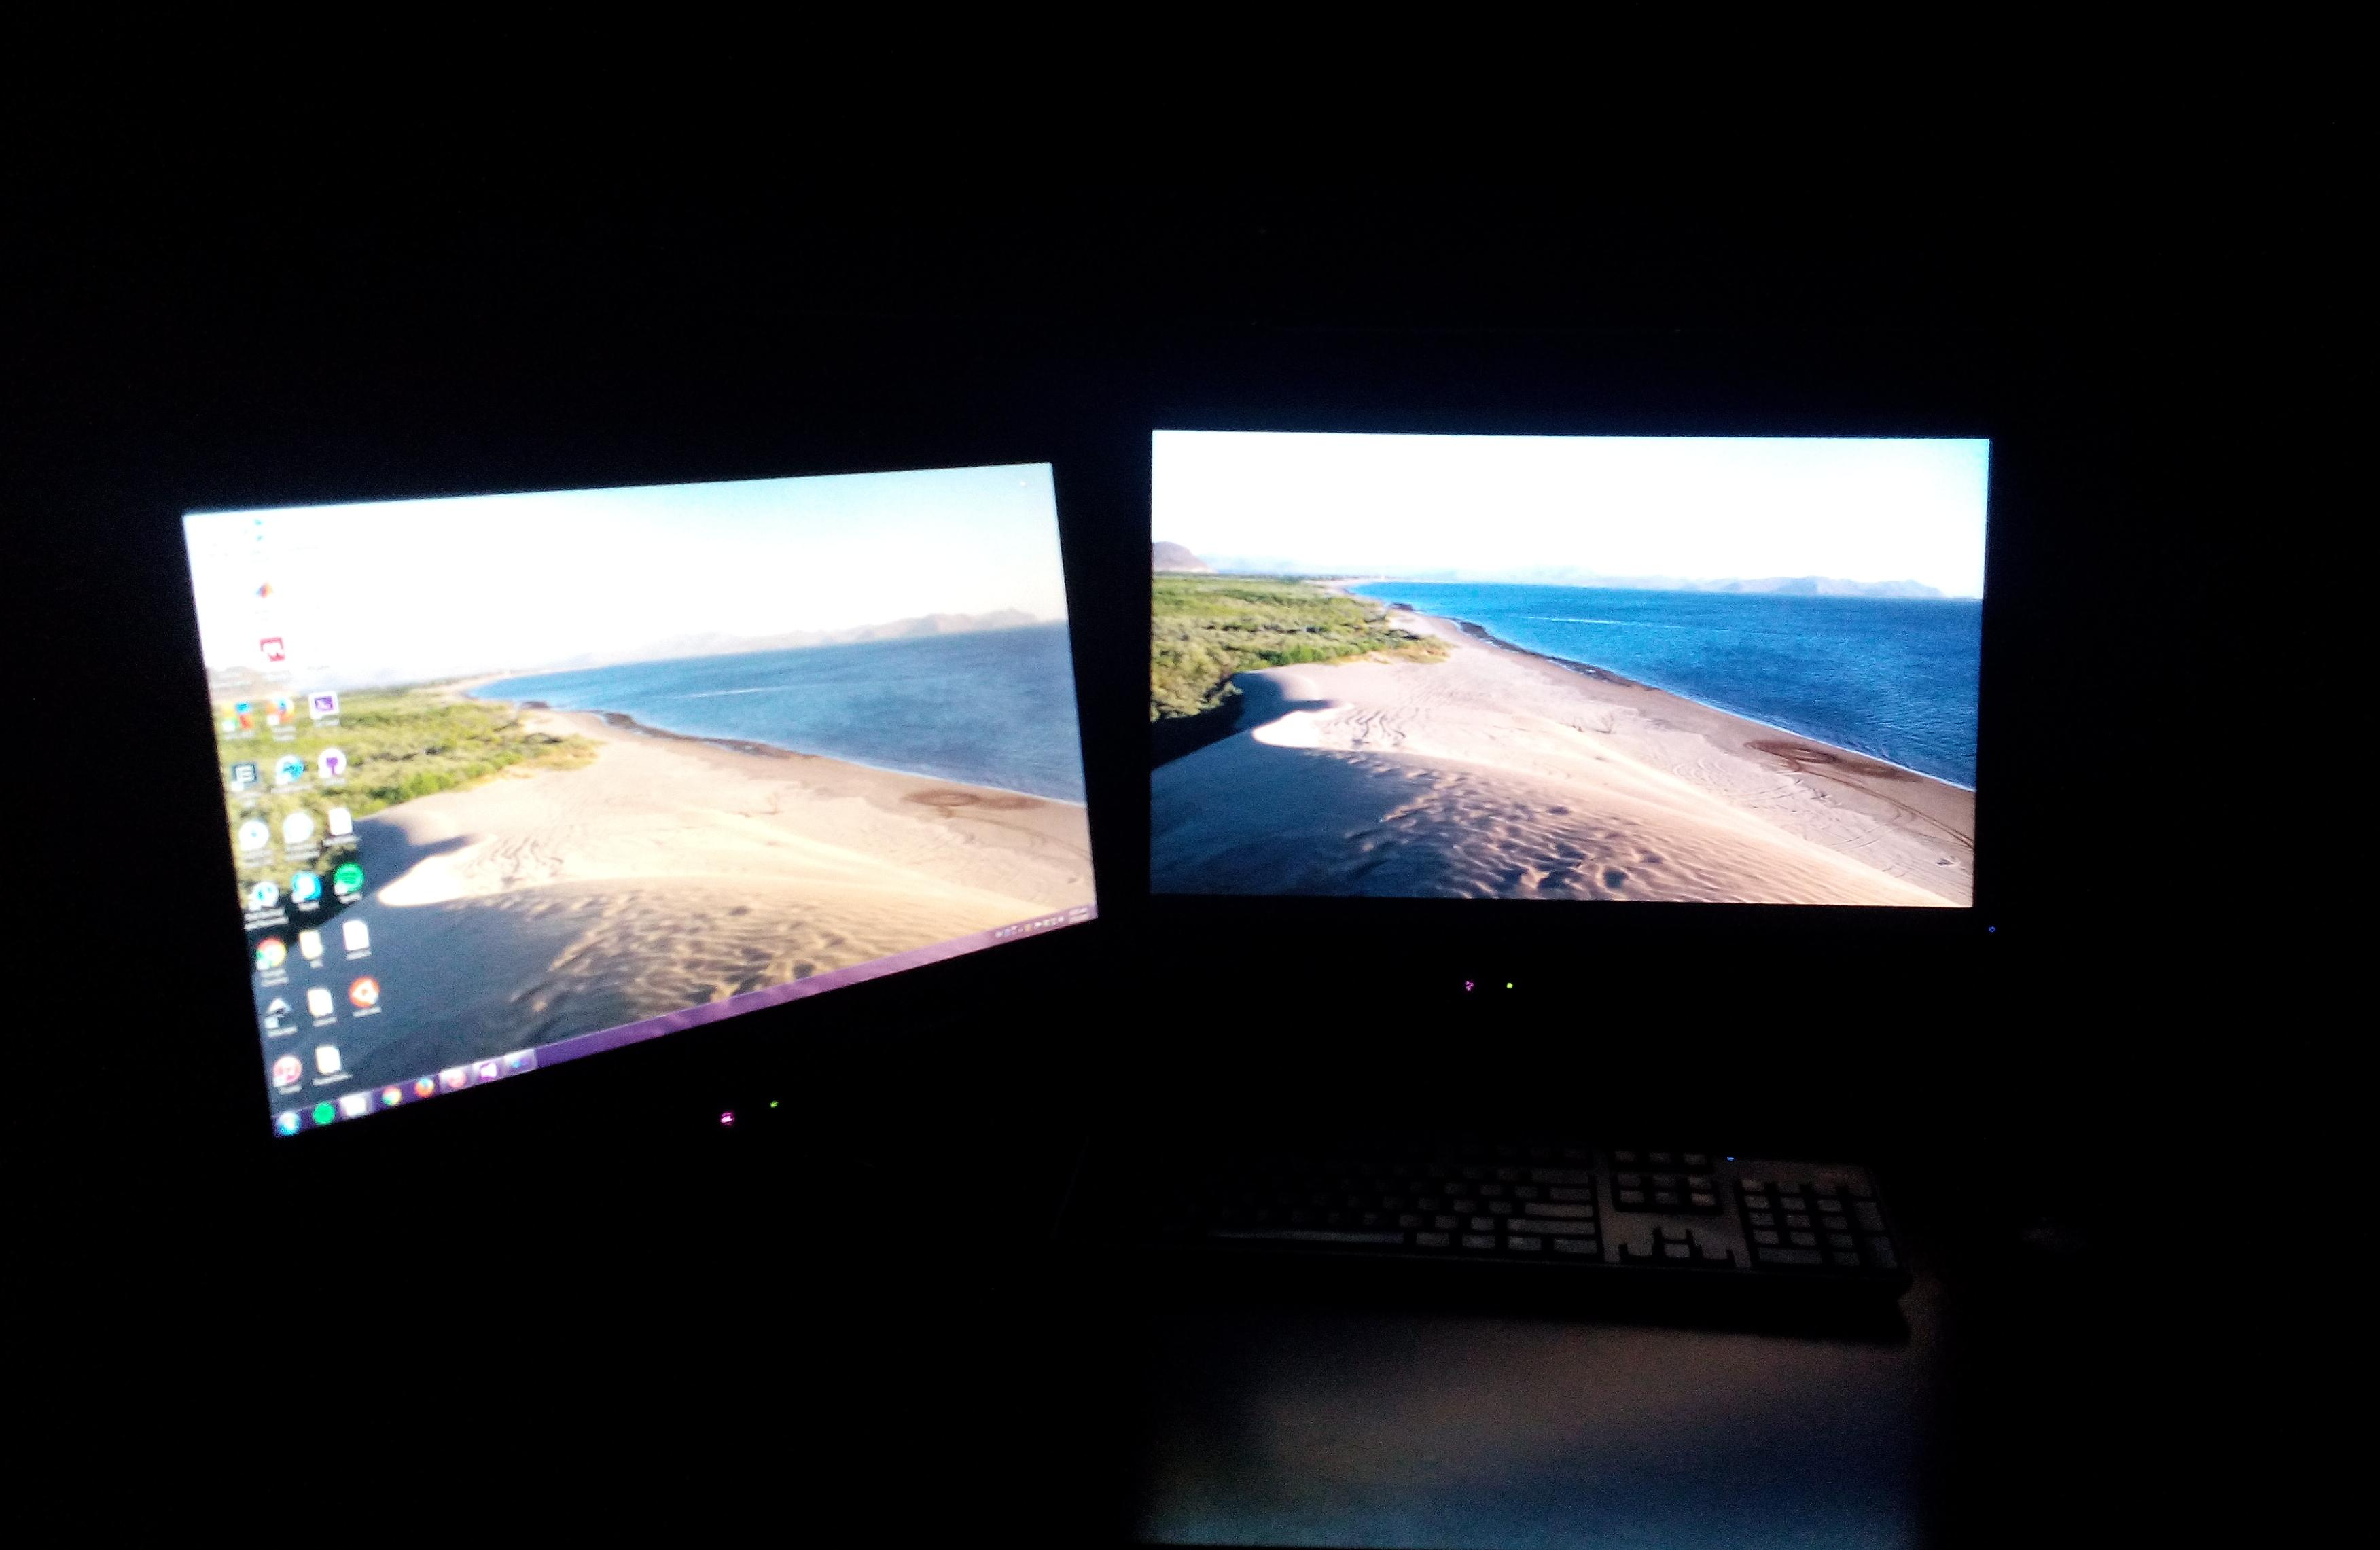
\includegraphics[scale=0.09]{./Figures/noIluminacion.jpg}
\end{center}
\caption{Laboratorio en condiciones con baja iluminación.}
\label{fig:LabNoIluminado} 
\end{figure} 

%---- 

\begin{itemize}

\item En el primer experimento el usuario esta a una distancia de $70$ $cm$ del Kinect frontal. En la Tabla \ref{table:70LnoK2} se encuentran los resultados del reconocimiento de los dos gestos utilizando los dos dispositivos y en la Tabla \ref{table:70LnoK1} los resultados usando un dispositivo.   

%\begin{figure}[h!]
%\centering
%\subfigure[Gesto 1 vista desde el Kinect frontal]{
\includegraphics[scale=.3]{./Figures/pusheen}\label{fig:iluminacionNo70:1}}
%\subfigure[Gesto 1 vista desde el Kinect lateral]{
\includegraphics[scale=.3]{./Figures/pusheen}\label{fig:iluminacionNo70:2}}
%\subfigure[Gesto 2 vista desde Kinect frontal]{
\includegraphics[scale=.3]{./Figures/pusheen}\label{fig:iluminacionNo70:3}}
%\subfigure[Gesto 2 vista desde Kinect lateral]{
\includegraphics[scale=.3]{./Figures/pusheen}\label{fig:iluminacionNo70:4}}
%\caption{Ejemplo de la imagenes capturadas a una distancia de $70$ $cm$.} \label{fig:iluminacionNo70}
%\end{figure}

\begin{table}[h!] 
\begin{center} 
\caption{Matriz de confusión del experimento sin iluminación, a una distancia de 70 cm utilizando ambos Kinect.} 
\label{table:70LnoK2}
\renewcommand{\arraystretch}{1.2}
\begin{tabular}{ r || c  c } 
 
        & \textbf{Gesto 1} & \textbf{Gesto 2} \\ \hline \hline  
\textbf{Gesto 1} & 190     &  110     \\ \hline  
\textbf{Gesto 2} & 196     &  4     \\   

\end{tabular}
\end{center} 
\end{table}  

La matriz de confusión muestra que $190$ gestos de la clase 1 y $4$ de la clase 2 fueron clasificados correctamente. De manera que se obtuvo una tasa de exactitud de $48.5 \%$ 

\begin{table}[h!] 
\begin{center} 
\caption{Matriz de confusión del experimento sin iluminación, a una distancia de 70 cm utilizando el Kinect frontal.}
\label{table:70LnoK1} 
\renewcommand{\arraystretch}{1.2}
\begin{tabular}{ r || c  c } 
        & \textbf{Gesto 1} & \textbf{Gesto 2} \\ \hline \hline  
\textbf{Gesto 1} & 154     &  46     \\ \hline  
\textbf{Gesto 2} & 167     &  33     \\   
\end{tabular}
\end{center} 
\end{table}  

La matriz de confusión muestra que $154$ gestos de la clase 1 y $133$ de la clase 2 fueron clasificados correctamente. De manera que se obtuvo una tasa de exactitud de $46.75 \%$ 

%---- 

\item En el segundo experimento el usuario est\'a a una distancia de $80$ $cm$ del Kinect frontal. En la Tabla \ref{table:80LnoK2} se encuentran los resultados del reconocimiento de los dos gestos utilizando los dos dispositivos, y en la Tabla \ref{table:80LnoK1} los resultados usando un dispositivo.   

%\begin{figure}[h!]
%\centering
%\subfigure[Gesto 1 vista desde el Kinect frontal]{
\includegraphics[scale=.3]{./Figures/pusheen}\label{fig:iluminacionNo80:1}}
%\subfigure[Gesto 1 vista desde el Kinect lateral]{
\includegraphics[scale=.3]{./Figures/pusheen}\label{fig:iluminacionNo80:2}}
%\subfigure[Gesto 2 vista desde Kinect frontal]{
\includegraphics[scale=.3]{./Figures/pusheen}\label{fig:iluminacionNo80:3}}
%\subfigure[Gesto 2 vista desde Kinect lateral]{
\includegraphics[scale=.3]{./Figures/pusheen}\label{fig:iluminacionNo80:4}}
%\caption{Ejemplo de la imagenes capturadas a una distancia de $80$ $cm$.} \label{fig:iluminacionNo80}
%\end{figure}

\begin{table}[h!] 
\begin{center} 
\caption{Matriz de confusión del experimento sin iluminación, a una distancia de 80 cm utilizando ambos Kinect.}
\label{table:80LnoK2} 
\renewcommand{\arraystretch}{1.2}
\begin{tabular}{ r || c  c } 
 
        & \textbf{Gesto 1} & \textbf{Gesto 2} \\ \hline \hline  
\textbf{Gesto 1} & 187     &  13     \\ \hline  
\textbf{Gesto 2} & 90     &  110     \\   

\end{tabular}
\end{center} 
\end{table}  

La matriz de confusión muestra que $187$ gestos de la clase 1 y $110$ de la clase 2 fueron clasificados correctamente. De manera que se obtuvo una tasa de exactitud de $74.25 \%$ 

\begin{table}[h!] 
\begin{center} 
\caption{Matriz de confusión del experimento sin iluminación, a una distancia de 80 cm utilizando el Kinect frontal.}
\label{table:80LnoK1}
\renewcommand{\arraystretch}{1.2}
\begin{tabular}{ r || c  c } 
 
        & \textbf{Gesto 1} & \textbf{Gesto 2} \\ \hline \hline  
\textbf{Gesto 1} & 162     &  37     \\ \hline  
\textbf{Gesto 2} & 4     &  166     \\   
\end{tabular}
\end{center} 
\end{table} 

La matriz de confusión muestra que $162$ gestos de la clase 1 y $166$ de la clase 2 fueron clasificados correctamente. De manera que se obtuvo una tasa de exactitud de $88.8\%$  

En este caso se obtiene una mayor exactitud utilizando un Kinect, sin embargo se observa que el uso de dos dispositivos ayuda a clasificar mejor el Gesto 1, pues se tiene mayor información con la cual se puede saber si es una palma con los dedos extendidos o solo es ruido proveniente del sensor.

%---

\item En el tercer experimento el usuario est\'a a una distancia de $90$ $cm$ del Kinect frontal. En la Tabla \ref{table:90LnoK2} se encuentran los resultados del reconocimiento de los dos gestos utilizando los dos dispositivos y en la Tabla \ref{table:90LnoK1} los resultados usando un dispositivo.    

%\begin{figure}[h!]
%\centering
%\subfigure[Gesto 1 vista desde el Kinect frontal]{
\includegraphics[scale=.3]{./Figures/pusheen}\label{fig:iluminacionNo90:1}}
%\subfigure[Gesto 1 viata desde el Kinect lateral]{
\includegraphics[scale=.3]{./Figures/pusheen}\label{fig:iluminacionNo90:2}}
%\subfigure[Gesto 2 vista desde Kinect frontal]{
\includegraphics[scale=.3]{./Figures/pusheen}\label{fig:iluminacionNo90:3}}
%\subfigure[Gesto 2 vista desde Kinect lateral]{
\includegraphics[scale=.3]{./Figures/pusheen}\label{fig:iluminacionNo90:4}}
%\caption{Ejemplo de la imagenes capturadas a una distancia de $90$ $cm$.} \label{fig:iluminacionNo70}
%\end{figure}

\begin{table}[h!] 
\begin{center}
\caption{Matriz de confusión del experimento sin iluminación, a una distancia de 90 cm utilizando ambos Kinect.}
\label{table:90LnoK2} 
\renewcommand{\arraystretch}{1.2}
\begin{tabular}{ r || c  c } 
        & \textbf{Gesto 1} & \textbf{Gesto 2} \\ \hline \hline  
\textbf{Gesto 1} & 150     &  50     \\ \hline  
\textbf{Gesto 2} & 6      &  194     \\   
\end{tabular}
\end{center} 
\end{table}

La matriz de confusión muestra que $150$ gestos de la clase 1 y $194$ de la clase 2 fueron clasificados correctamente. De manera que se obtuvo una tasa de exactitud de $86 \%$ 

\begin{table}[h!] 
\begin{center}
\caption{Matriz de confusión del experimento sin iluminación, a una distancia de 90 cm utilizando el Kinect frontal.}
\label{table:90LnoK1} 
\renewcommand{\arraystretch}{1.2}
\begin{tabular}{ r || c  c } 
 
        & \textbf{Gesto 1} & \textbf{Gesto 2} \\ \hline \hline  
\textbf{Gesto 1} & 138     &  61     \\ 
\end{tabular}
\end{center} 
\end{table} 

En el caso cuando se toma como entrada solo un Kinect, al igual que en el experimento de iluminación media y con distancia también de $90$ $cm$. Solo se detectaron los gestos de la clase 1, de los cuales se clasificaron correctamente $138$ de $199$ detectados. 

En este experimento se observa que hay mayor exactitud en el reconocimiento utilizando dos Kinect y al igual que en la mayoría de los casos, hay un error mayor en la clasificación de la clase 1. 


\end{itemize}

Los experimentos explicados anteriormente muestran que el Gesto 1 produce un error mayor, debido a la resolución de sensor, pues no en todas las imágenes la mano est\'a completa, en los casos que no est\'a completamente vista por el sensor frontal y logra ser detectada por el sensor lateral con información favorable, es cuando se puede apreciar una mayor exactitud de reconocimiento usando ambos Kinect. 
Ser\'ia conveniente hacer un experimento donde las imágenes tengan una buena resolución y ninguna obstrucción para validar el rendimiento del sistema. Debido a que la imágenes utilizadas no eran ideales pues contenían  ruido o obstrucciones. Se decidió hacer este tipo de pruebas para lograr resultados m\'as apegados a la realidad es decir en ambientes naturales. 
  

%:::::::::::::::::::::::::::::::::::::::::::::::::::::::::::::::::::::::::::::::::::::::::::::::::::::::::::::::::


\section{Experimentos de gestos dinámicos}\label{TestDinamicGestures} 

La evaluación del sistema en cuanto al reconocimiento de los gestos dinámicos se realiz\'o de la siguiente forma: al igual que en los gestos estáticos se hicieron dos conjuntos de experimentos cada uno con diferentes tipos de iluminación, media y sin iluminación. En cada conjunto de experimentos se tom\'o en cuenta la distancia, debido a que en cada grupo se analizaron tres distancias, $70$, $80$, $90$ $cm$. 

Los gestos analizados fueron dos. El primero corresponde a la palma de la mano con los dedos separados, Gesto 3, en movimiento y el segundo el puño de la mano, Gesto 4, también en movimiento. Los gestos fueron realizados por tres usuarios distintos. Para cada experimento se realizaron cinco repeticiones de cada gesto y cada uno tenia una duración de treinta cuadros por segundo. Se tom\'o como gesto v\'alido si el porcentaje de reconocimiento de cada gestos estático presente en cada segundo es mayor o igual a $80 \%$, esto con base al trabajo realizado por \citep{Sultana2012}. 
También se prob\'o el sistema usando un solo Kinect, el frontal, en las mismas circunstancias mencionadas anteriormente. 
Enseguida se presentan los resultados de cada experimento realizado, por usuario. 


\subsection{Experimentos con iluminación media} 
Para el conjunto de estos experimentos, las imágenes se capturaron en un laboratorio con iluminación media, véase la Figura \ref{fig:LabMedioIluminado}.

\begin{itemize}

\item En el primer experimento el usuario est\'a a una distancia de $70$ $cm$ del Kinect frontal. En la Tabla \ref{table:D70LK1} se encuentran los resultados del reconocimiento de los dos gestos utilizando solo el Kinect frontal. En la Tabla \ref{table:D70LK2} se presentan los resultados utilizando los dos dispositivos Kinect.  

\begin{table}[h!]
\begin{center} 
\caption{Precisión de gestos realizados en un ambiente de iluminación media a una distancia de 70 cm utilizando el Kinect frontal. P1, P2 y P3 representan a los participantes, G3 y G4 representan el Gesto 3 y Gesto 4 respectivamente, R1, R2, R3, R4 y R5 representa el número de repeticiones.} 
\label{table:D70LK1} 
\renewcommand{\arraystretch}{1.2}
\setlength{\tabcolsep}{17pt}
\begin{tabular}{ c  c || c  c  c  c  c  } 
\hline 
\multicolumn{7}{ c }{\textbf{Porcentajes de precisión del reconocimiento de cada repetición.}}\\ \cline{1-7}
\multicolumn{2}{ c }{} & \textbf{R1} & \textbf{R2} & \textbf{R3} & \textbf{R4}  & \textbf{R5}\\  \cline{3-7} \hline\hline
{\multirow{2}{*}{\textbf{P1}}} & {G3} & 77 & 80 & 83 & 73 & 70 \\ \cline{2-7}
                               & {G4} & 93 & 100 & 100 & 93 & 97 \\ \hline \hline
{\multirow{2}{*}{\textbf{P2}}} & {G3} & 87 & 80 & 87 & 70 & 97 \\ \cline{2-7}
                      		   & {G4} & 97 & 93 & 97 & 93 & 93 \\ \hline \hline
{\multirow{2}{*}{\textbf{P3}}} & {G3} & 83 & 100 & 80 & 53 & 90 \\ \cline{2-7}
                      		   & {G4} & 100 & 93 & 93 & 87 & 100 \\ \hline
\end{tabular}
\end{center} 
\end{table} 

En la tabla \ref{table:D70LK1} se observa que arriba del $90 \%$ de los gestos realizados por cada participante son reconocidos correctamente. A excepción del participante uno al realizar el Gesto 3, pues solo reconoció dos gestos dinámicos de los cinco realizados. Esto se debe al sensor, pues las manos del participante uno no son tan grandes y el sensor no logra captar en todas la imágenes los dedos del participante. 

\begin{table}[h!]
\begin{center} 
\caption{Precisión de gestos realizados en un ambiente de iluminación media a una distancia de 70 cm utilizando ambos Kinect. P1, P2 y P3 representan a los participantes, G3 y G4 representan el Gesto 3 y Gesto 4 respectivamente, R1, R2, R3, R4 y R5 representa el número de repeticiones.}
\label{table:D70LK2}
\renewcommand{\arraystretch}{1.2}
\setlength{\tabcolsep}{17pt}
\begin{tabular}{ c  c || c  c  c  c  c  } 
\hline
\multicolumn{7}{ c }{\textbf{Porcentajes de precisión del reconocimiento de cada repetición.}}\\ \cline{1-7}
\multicolumn{2}{ c }{} &\textbf{R1} & \textbf{R2} & \textbf{R3} & \textbf{R4}  & \textbf{R5}\\ \cline{1-7} \hline\hline
{\multirow{1}{*}{\textbf{P1}}} & {G3} & 73 & 63 & 77 & 73 & 63 \\ \cline{2-7} \hline \hline
{\multirow{2}{*}{\textbf{P2}}} & {G3} & 100 & 93 & 87 & 93 & 87 \\ \cline{2-7}
                      & {G4} & 93 & 77 & 77 & 67 & 60 \\ \hline \hline
{\multirow{2}{*}{\textbf{P3}}} & {G3} & 100 & 100 & 93 & 97 & 93 \\ \cline{2-7}
                      & {G4} & 73 & 90 & 83 & 63 & 83 \\ \hline
\end{tabular}  
\end{center} 
\end{table} 

Al utilizar ambos Kinect se observa que hay menor exactitud de reconocimiento de los gestos. C\'omo se usan las mismas imágenes para uno y dos Kinect en cada prueba, se tiene la misma justificación en la exactitud del participante uno. 
%---

\item En el segundo experimento el usuario est\'a a una distancia de $80$ $cm$ del Kinect frontal. En la Tabla \ref{table:D80LK1} se encuentran los resultados del reconocimiento de los dos gestos utilizando solo el Kinect frontal. En la Tabla \ref{table:D80LK2} se presentan los resultados utilizando los dos dispositivos Kinect.   

%\begin{figure}[h!]
%\centering
%\subfigure[Cuadro inicial]{
\includegraphics[scale=.3]{./Figures/pusheen}\label{fig:G1IM80:1}}
%\subfigure[Cuadro número 20]{
\includegraphics[scale=.3]{./Figures/pusheen}\label{fig:G1IM80:2}}
%\subfigure[Cuadro número 40]{
\includegraphics[scale=.3]{./Figures/pusheen}\label{fig:G1IM80:3}}
%\subfigure[Cuadro final]{
\includegraphics[scale=.3]{./Figures/pusheen}\label{fig:G1IM80:4}}
%\caption{Gesto de la palma con los dedos abiertas a $80$ $cm$.} \label{fig:G1I80}
%\end{figure}
%
%\begin{figure}[h!]
%\centering
%\subfigure[Cuadro inicial]{
\includegraphics[scale=.3]{./Figures/pusheen}\label{fig:G2IM80:1}}
%\subfigure[Cuadro número 20]{
\includegraphics[scale=.3]{./Figures/pusheen}\label{fig:G2IM80:2}}
%\subfigure[Cuadro número 40]{
\includegraphics[scale=.3]{./Figures/pusheen}\label{fig:G2IM80:3}}
%\subfigure[Cuadro final]{
\includegraphics[scale=.3]{./Figures/pusheen}\label{fig:G2IM80:4}}
%\caption{Gesto del puño de la mano a $80$ $cm$.} \label{fig:G2I80}
%\end{figure}

% 1 kinect 80 LM 
\begin{table}[h!]
\begin{center} 
\caption{Precisión de gestos realizados en un ambiente de iluminación media a una distancia de 80 cm utilizando el Kinect frontal. P1, P2 y P3 representan a los participantes, G3 y G4 representan el Gesto 3 y Gesto 4 respectivamente, R1, R2, R3, R4 y R5 representa el número de repeticiones.} 
\label{table:D80LK1}
\renewcommand{\arraystretch}{1.2}
\setlength{\tabcolsep}{17pt}
\begin{tabular}{ c  c || c  c  c  c  c  } 
\hline
\multicolumn{7}{ c }{\textbf{Porcentajes de precisión del reconocimiento de cada repetición.}}\\ \cline{1-7}
\multicolumn{2}{ c }{} &\textbf{R1} & \textbf{R2} & \textbf{R3} & \textbf{R4}  & \textbf{R5}\\ \cline{1-7} \hline\hline
{\multirow{2}{*}{\textbf{P1}}} & {G3} & 33 & 27 & 30 & 50 & 57 \\ \cline{2-7}
                      & {G4} & 100 & 100 & 70 & 87 & 77 \\ \hline \hline
{\multirow{2}{*}{\textbf{P2}}} & {G3} & 37 & 27 & 33 & 38 & 29 \\ \cline{2-7}
                      & {G4} & 100 & 93 & 90 & 80 & 75 \\ \hline \hline
{\multirow{2}{*}{\textbf{P3}}} & {G3} & 47 & 87 & 60 & 60 & 63 \\ \cline{2-7}
                      & {G4} & 100 & 90 & 97 & 92 & 95 \\ \hline
\end{tabular} 
\end{center} 
\end{table}

\begin{table}[h!]
\begin{center} 
\caption{Precisión de gestos realizados en un ambiente de iluminación media a una distancia de 80 cm utilizando ambos Kinect. P1, P2 y P3 representan a los participantes, G3 y G4 representan el Gesto 3 y Gesto 4 respectivamente, R1, R2, R3, R4 y R5 representa el número de repeticiones.} 
\label{table:D80LK2}
\renewcommand{\arraystretch}{1.2}
\setlength{\tabcolsep}{17pt}
\begin{tabular}{ c  c || c  c  c  c  c  } 
\hline
\multicolumn{7}{ c }{\textbf{Porcentajes de precisión del reconocimiento de cada repetición.}}\\ \cline{1-7}
\multicolumn{2}{ c }{} &\textbf{R1} & \textbf{R2} & \textbf{R3} & \textbf{R4}  & \textbf{R5}\\ \cline{1-7} \hline\hline
{\multirow{2}{*}{\textbf{P1}}} & {G3} & 83 & 86 & 67 & 87 & 70 \\ \cline{2-7}
                      & {G4} & 35 & 53 & 70 & 77 & 57 \\ \hline \hline
{\multirow{2}{*}{\textbf{P2}}} & {G3} & 33 & 57 & 57 & 73 & 60 \\ \cline{2-7}
                      & {G4} & 93 & 93 & 90 & 90 & 80 \\ \hline \hline
{\multirow{2}{*}{\textbf{P3}}} & {G3} & 93 & 100 & 67 & 100 & 80 \\ \cline{2-7}
                      & {G4} & 100 & 93 & 87 & 83 & 90 \\ \hline
\end{tabular}
\end{center} 
\end{table} 

Para ambas pruebas con uno y dos Kinect se obtuvieron resultados similares, desafortunadamente hubo mayores casos de reconocimiento fallido, en especial cuando se realiza el Gesto 3. Aquí se puede observar un mejor reconocimiento con el uso de ambos Kinect.

%---

\item En el tercer experimento el usuario est\'a a una distancia de $90$ $cm$ del Kinect frontal. En la Tabla \ref{table:D90LK1} se encuentran los resultados del reconocimiento de los dos gestos utilizando solo el Kinect frontal. En la Tabla \ref{table:D90LK2} se presentan los resultados utilizando los dos dispositivos Kinect.    

%\begin{figure}[h!]
%\centering
%\subfigure[Cuadro inicial]{
\includegraphics[scale=.3]{./Figures/pusheen}\label{fig:G1IM90:1}}
%\subfigure[Cuadro número 20]{
\includegraphics[scale=.3]{./Figures/pusheen}\label{fig:G1IM90:2}}
%\subfigure[Cuadro número 40]{
\includegraphics[scale=.3]{./Figures/pusheen}\label{fig:G1IM90:3}}
%\subfigure[Cuadro final]{
\includegraphics[scale=.3]{./Figures/pusheen}\label{fig:G1IM90:4}}
%\caption{Gesto de la palma con los dedos abiertas $90$ $cm$.} \label{fig:G1IM90}
%\end{figure}
%
%\begin{figure}[h!]
%\centering
%\subfigure[Cuadro inicial]{
\includegraphics[scale=.3]{./Figures/pusheen}\label{fig:G2IM90:1}}
%\subfigure[Cuadro número 20]{
\includegraphics[scale=.3]{./Figures/pusheen}\label{fig:G2IM90:2}}
%\subfigure[Cuadro número 40]{
\includegraphics[scale=.3]{./Figures/pusheen}\label{fig:G2IM90:3}}
%\subfigure[Cuadro final]{\includegraphics[scale=.3]{./Figures/pusheen}\label{fig:G2IM90:4}}
%\caption{Gesto del puño de la mano $90$ $cm$.} \label{fig:G2IM90}
%\end{figure}

\begin{table}[h!]
\begin{center} 
\caption{Precisión de gestos realizados en un ambiente de iluminación media a una distancia de 90 cm utilizando el Kinect frontal. P1, P2 y P3 representan a los participantes, G3 y G4 representan el Gesto 3 y Gesto 4 respectivamente, R1, R2, R3, R4 y R5 representa el número de repeticiones.} 
\label{table:D90LK1}
\renewcommand{\arraystretch}{1.2}
\setlength{\tabcolsep}{17pt}
\begin{tabular}{ c  c || c  c  c  c  c  } 
\hline
\multicolumn{7}{ c }{\textbf{Porcentajes de precisión del reconocimiento de cada repetición.}}\\ \cline{1-7}
\multicolumn{2}{ c }{} &\textbf{R1} & \textbf{R2} & \textbf{R3} & \textbf{R4}  & \textbf{R5}\\ \cline{1-7} \hline\hline
{\multirow{2}{*}{\textbf{P1}}} & {G3} & 87 & 87 & 53 & 87 & 67 \\ \cline{2-7}
                      & {G4} & 100 & 100 & 100 & 90 & 92 \\ \hline \hline
{\multirow{2}{*}{\textbf{P2}}} & {G3} & 87 & 87 & 90 & 93 & 80 \\ \cline{2-7}
                      & {G4} & 83 & 73 & 97 & 80 & 75 \\ \hline \hline
{\multirow{2}{*}{\textbf{P3}}} & {G3} & 90 & 97 & 97 & 100 & 90 \\ \cline{2-7}
                      & {G4} & 77 & 90 & 80 & 75 & 80 \\ \hline
\end{tabular}
\end{center} 
\end{table}

\begin{table}[h!]
\begin{center} 
\caption{Precisión de gestos realizados en un ambiente de iluminación media a una distancia de 90 cm utilizando ambos Kinect. P1, P2 y P3 representan a los participantes, G3 y G4 representan el Gesto 3 y Gesto 4 respectivamente, R1, R2, R3, R4 y R5 representa el número de repeticiones.} 
\label{table:D90LK2}
\renewcommand{\arraystretch}{1.2}
\setlength{\tabcolsep}{17pt}
\begin{tabular}{ c  c || c  c  c  c  c  } 
\hline
\multicolumn{7}{ c }{\textbf{Porcentajes de precisión del reconocimiento de cada repetición.}}\\ \cline{1-7}
\multicolumn{2}{ c }{} &\textbf{R1} & \textbf{R2} & \textbf{R3} & \textbf{R4}  & \textbf{R5}\\ \cline{1-7} \hline\hline
{\multirow{2}{*}{\textbf{P1}}} & {G3} & 30 & 37 & 13 & 13 & 30 \\ \cline{2-7}
                      & {G4} & 100 & 98 & 95 & 100 & 98 \\ \hline \hline
{\multirow{2}{*}{\textbf{P2}}} & {G3} & 50 & 60 & 67 & 70 & 75 \\ \cline{2-7}
                      & {G4} & 77 & 78 & 75 & 80 & 70 \\ \hline \hline
{\multirow{2}{*}{\textbf{P3}}} & {G3} & 77 & 73 & 80 & 97 & 90 \\ \cline{2-7}
                      & {G4} & 77 & 90 & 91 & 80 & 75 \\ \hline
\end{tabular}
\end{center}
\end{table}

En este caso el experimento mostró un mejor reconocimiento al usar un solo dispositivo, si existe gran diferencia en el uso de dos dispositivos generalmente en la realización del Gesto 3.

\end{itemize}


\subsection{Experimentos sin iluminación}
Para este experimento las imágenes se capturaron en un laboratorio sin iluminación, véase la Figura \ref{fig:LabNoIluminado}.

\begin{itemize}

\item En el primer experimento el usuario est\'a a una distancia de $70$ $cm$ del Kinect frontal. En la Tabla \ref{table:D70LMK1} se encuentran los resultados del reconocimiento de los dos gestos utilizando solo el Kinect frontal. En la Tabla \ref{table:D70LMK2} se presentan los resultados utilizando los dos dispositivos Kinect. 

%\begin{figure}[h!]
%\centering
%\subfigure[Cuadro inicial]{\includegraphics[scale=.3]{./Figures/pusheen}\label{fig:G1INO70:1}}
%\subfigure[Cuadro número 20]{\includegraphics[scale=.3]{./Figures/pusheen}\label{fig:G1INO70:2}}
%\subfigure[Cuadro número 40]{\includegraphics[scale=.3]{./Figures/pusheen}\label{fig:G1INO70:3}}
%\subfigure[Cuadro final]{\includegraphics[scale=.3]{./Figures/pusheen}\label{fig:G1INO70:4}}
%\caption{Gesto de la palma con los dedos abiertas a $70$ $cm$.} \label{fig:G1INO70}
%\end{figure}
%
%\begin{figure}[h!]
%\centering
%\subfigure[Cuadro inicial]{\includegraphics[scale=.3]{./Figures/pusheen}\label{fig:G2INO70:1}}
%\subfigure[Cuadro número 20]{\includegraphics[scale=.3]{./Figures/pusheen}\label{fig:G2INO70:2}}
%\subfigure[Cuadro número 40]{\includegraphics[scale=.3]{./Figures/pusheen}\label{fig:G2INO70:3}}
%\subfigure[Cuadro final]{\includegraphics[scale=.3]{./Figures/pusheen}\label{fig:G2INO70:4}}
%\caption{Gesto del puño de la mano a $70$ $cm$.} \label{fig:G2INO70}
%\end{figure}

\begin{table}[h!]
\begin{center} 
\caption{Precisión de gestos realizados en un ambiente sin iluminación a una distancia de 70 cm utilizando el Kinect frontal. P1, P2 y P3 representan a los participantes, G3 y G4 representan el Gesto 3 y Gesto 4 respectivamente, R1, R2, R3, R4 y R5 representa el número de repeticiones.} 
\label{table:D70LMK1}
\renewcommand{\arraystretch}{1.2}
\setlength{\tabcolsep}{17pt}
\begin{tabular}{ c  c || c  c  c  c  c  } 
\hline
\multicolumn{7}{ c }{\textbf{Porcentajes de precisión del reconocimiento de cada repetición.}}\\ \cline{1-7}
\multicolumn{2}{ c }{} &\textbf{R1} & \textbf{R2} & \textbf{R3} & \textbf{R4}  & \textbf{R5}\\ \cline{1-7} \hline\hline
{\multirow{2}{*}{\textbf{P1}}} & {G3} & 77 & 80 & 57 & 70 & 60 \\ \cline{2-7}
                      & {G4} & 100 & 97 & 93 & 100 & 97 \\ \hline \hline
{\multirow{2}{*}{\textbf{P2}}} & {G3} & 97 & 57 & 80 & 53 & 87 \\ \cline{2-7}
                      & {G4} & 100 & 97 & 83 & 87 & 87 \\ \hline \hline
{\multirow{2}{*}{\textbf{P3}}} & {G3} & 73 & 43 & 43 & 47 & 60 \\ \cline{2-7}
                      & {G4} & 100 & 93 & 97 & 93 & 93 \\ \hline
\end{tabular}
\end{center} 
\end{table}

\begin{table}[h!]
\begin{center} 
\caption{Precisión de gestos realizados en un ambiente sin iluminación a una distancia de 70 cm utilizando ambos Kinect. P1, P2, P3 representan a los participantes, R1, R2, R3, R4, R5 representan el número de repeticiones} 
\label{table:D70LMK2}
\renewcommand{\arraystretch}{1.2}
\setlength{\tabcolsep}{17pt}
\begin{tabular}{ c  c || c  c  c  c  c  } 
\hline
\multicolumn{7}{ c }{\textbf{Porcentajes de precisión del reconocimiento de cada repetición.}}\\ \cline{1-7}
\multicolumn{2}{ c }{} &\textbf{R1} & \textbf{R2} & \textbf{R3} & \textbf{R4}  & \textbf{R5}\\ \cline{1-7} \hline\hline
{\multirow{2}{*}{\textbf{P1}}} & {G3} & 93 & 83 & 100 & 77 & 87 \\ \cline{2-7}
                      & {G4} & 100 & 100 & 97 & 97 & 100 \\ \hline \hline
{\multirow{2}{*}{\textbf{P2}}} & {G3} & 97 & 97 & 87 & 93 & 97 \\ \cline{2-7}
                      & {G4} & 80 & 93 & 90 & 97 & 97 \\ \hline \hline
{\multirow{2}{*}{\textbf{P3}}} & {G3} & 83 & 87 & 97 & 97 & 100 \\ \cline{2-7}
                      & {G4} & 100 & 97 & 93 & 87 & 90 \\ \hline
\end{tabular}
\end{center} 
\end{table}


Analizando cada repetición de cada gesto se observa que una mayor reconocimiento cuando se utilizan los dos dispositivos, en especial cuando se reconoce el Gesto 3 de los participantes uno y tres. 

%---

\item En el segundo experimento el usuario est\'a a una distancia de $80$ $cm$ del Kinect frontal. En la Tabla \ref{table:D80LMK1} se encuentran los resultados del reconocimiento de los dos gestos utilizando solo el Kinect frontal. En la Tabla \ref{table:D80LMK2} se presentan los resultados utilizando los dos dispositivos Kinect.    

%\begin{figure}[h!]
%\centering
%\subfigure[Cuadro inicial]{\includegraphics[scale=.3]{./Figures/pusheen}\label{fig:G1INO80:1}}
%\subfigure[Cuadro número 20]{\includegraphics[scale=.3]{./Figures/pusheen}\label{fig:G1INO80:2}}
%\subfigure[Cuadro número 40]{\includegraphics[scale=.3]{./Figures/pusheen}\label{fig:G1INOM80:3}}
%\subfigure[Cuadro final]{\includegraphics[scale=.3]{./Figures/pusheen}\label{fig:G1INO80:4}}
%\caption{Gesto de la palma con los dedos abiertas a $80$ $cm$.} \label{fig:G1NO80}
%\end{figure}
%
%\begin{figure}[h!]
%\centering
%\subfigure[Cuadro inicial]{\includegraphics[scale=.3]{./Figures/pusheen}\label{fig:G2INO80:1}}
%\subfigure[Cuadro número 20]{\includegraphics[scale=.3]{./Figures/pusheen}\label{fig:G2INO80:2}}
%\subfigure[Cuadro número 40]{\includegraphics[scale=.3]{./Figures/pusheen}\label{fig:G2INO80:3}}
%\subfigure[Cuadro final]{\includegraphics[scale=.3]{./Figures/pusheen}\label{fig:G2INO80:4}}
%\caption{Gesto del puño de la mano a $80$ $cm$.} \label{fig:G2INO80}
%\end{figure}

\begin{table}[h!]
\begin{center} 
\caption{Precisión de gestos realizados en un ambiente sin iluminación a una distancia de 80 cm utilizando el Kinect frontal. P1, P2, P3 representan a los participantes, R1, R2, R3, R4, R5 representan el número de repeticiones} 
\label{table:D80LMK1}
\renewcommand{\arraystretch}{1.2}
\setlength{\tabcolsep}{17pt}
\begin{tabular}{ c  c || c  c  c  c  c  } 
\hline
\multicolumn{7}{ c }{\textbf{Porcentajes de precisión del reconocimiento de cada repetición.}}\\ \cline{1-7}
\multicolumn{2}{ c }{} &\textbf{R1} & \textbf{R2} & \textbf{R3} & \textbf{R4}  & \textbf{R5}\\ \cline{1-7} \hline\hline
{\multirow{2}{*}{\textbf{P1}}} & {G3} & 57 & 63 & 60 & 63 & 63 \\ \cline{2-7}
                      & {G4} & 100 & 100 & 100 & 100 & 100 \\ \hline \hline
{\multirow{2}{*}{\textbf{P2}}} & {G3} & 40 & 43 & 60 & 70 & 75 \\ \cline{2-7}
                      & {G4} & 100 & 93 & 97 & 93 & 98 \\ \hline \hline
{\multirow{2}{*}{\textbf{P3}}} & {G3} & 80 & 87 & 67 & 77 & 63 \\ \cline{2-7}
                      & {G4} & 97 & 87 & 100 & 90 & 87 \\ \hline
\end{tabular}
\end{center} 
\end{table}

\begin{table}[h!]
\begin{center} 
\caption{Precisión de gestos realizados en un ambiente sin iluminación a una distancia de 80 cm utilizando ambos Kinect. P1, P2 y P3 representan a los participantes, G3 y G4 representan el Gesto 3 y Gesto 4 respectivamente, R1, R2, R3, R4 y R5 representa el número de repeticiones.} 
\label{table:D80LMK2}
\renewcommand{\arraystretch}{1.2}
\setlength{\tabcolsep}{17pt}
\begin{tabular}{ c  c || c  c  c  c  c  } 
\hline
\multicolumn{7}{ c }{\textbf{Porcentajes de precisión del reconocimiento de cada repetición.}}\\ \cline{1-7}
\multicolumn{2}{ c }{} &\textbf{R1} & \textbf{R2} & \textbf{R3} & \textbf{R4}  & \textbf{R5}\\ \cline{1-7} \hline\hline
{\multirow{2}{*}{\textbf{P1}}} & {G3} & 63 & 70 & 90 & 80 & 77 \\ \cline{2-7}
                      & {G4} & 87 & 100 & 93 & 90 & 93 \\ \hline \hline
{\multirow{2}{*}{\textbf{P2}}} & {G3} & 60 & 73 & 47 & 63 & 73 \\ \cline{2-7}
                      & {G4} & 100 & 97 & 87 & 90 & 90 \\ \hline \hline
{\multirow{2}{*}{\textbf{P3}}} & {G3} & 87 & 100 & 73 & 83 & 80 \\ \cline{2-7}
                      & {G4} & 73 & 73 & 93 & 83 & 93 \\ \hline 
\end{tabular}
\end{center}
\end{table} 

En este experimento se puede observar que las repeticiones del Gesto 4 con cada participante obtienen mayor precisi\'on utilizando un Kinect. En este caso se observa que el Gesto 3 no es clasificado correctamente en la mayoría de las repeticiones de los tres participantes a excepción del participante tres, que muestra mayor desempeño cuando se utilizan los dos dispositivos.

%--

\item En el tercer experimento el usuario est\'a a una distancia de $90$ $cm$ del Kinect frontal. En la Tabla \ref{table:D90LMK1} se encuentran los resultados del reconocimiento de los dos gestos utilizando solo el Kinect frontal. En la Tabla \ref{table:D90LMK2} se presentan los resultados utilizando los dos dispositivos Kinect.     

%\begin{figure}[h!]
%\centering
%\subfigure[Cuadro inicial]{\includegraphics[scale=.3]{./Figures/pusheen}\label{fig:G1INO90:1}}
%\subfigure[Cuadro número 20]{\includegraphics[scale=.3]{./Figures/pusheen}\label{fig:G1INO90:2}}
%\subfigure[Cuadro número 40]{\includegraphics[scale=.3]{./Figures/pusheen}\label{fig:G1INO90:3}}
%\subfigure[Cuadro final]{\includegraphics[scale=.3]{./Figures/pusheen}\label{fig:G1INO90:4}}
%\caption{Gesto de la palma con los dedos abiertas $90$ $cm$.} \label{fig:G1INO90}
%\end{figure}
%
%\begin{figure}[h!]
%\centering
%\subfigure[Cuadro inicial]{\includegraphics[scale=.3]{./Figures/pusheen}\label{fig:G2INO90:1}}
%\subfigure[Cuadro número 20]{\includegraphics[scale=.3]{./Figures/pusheen}\label{fig:G2INO90:2}}
%\subfigure[Cuadro número 40]{\includegraphics[scale=.3]{./Figures/pusheen}\label{fig:G2INO90:3}}
%\subfigure[Cuadro final]{\includegraphics[scale=.3]{./Figures/pusheen}\label{fig:G2INO90:4}}
%\caption{Gesto del puño de la mano $90$ $cm$.} \label{fig:G2INO90}
%\end{figure}

\begin{table}[h!]
\begin{center} 
\caption{Precisión de gestos realizados en un ambiente sin iluminación a una distancia de 90 cm utilizando el Kinect frontal. P1, P2 y P3 representan a los participantes, G3 y G4 representan el Gesto 3 y Gesto 4 respectivamente, R1, R2, R3, R4 y R5 representa el número de repeticiones.} 
\label{table:D90LMK1}
\renewcommand{\arraystretch}{1.2}
\setlength{\tabcolsep}{17pt}
\begin{tabular}{ c  c || c  c  c  c  c  } 
\hline
\multicolumn{7}{ c }{\textbf{Porcentajes de precisión del reconocimiento de cada repetición.}}\\ \cline{1-7}
\multicolumn{2}{ c }{} & \textbf{R1} & \textbf{R2} & \textbf{R3} & \textbf{R4}  & \textbf{R5}\\ \cline{1-7} \hline\hline
{\multirow{1}{*}{\textbf{P1}}} & {G3} & 57 & 70 & 70 & 67 & 77 \\ \cline{2-7}\hline\hline
{\multirow{2}{*}{\textbf{P2}}} & {G3} & 70 & 80 & 80 & 77 & 80 \\ \cline{2-7}
                      & {G4} & 73 & 80 & 83 & 97 & 80 \\ \hline \hline
{\multirow{2}{*}{\textbf{P3}}} & {G3} & 70 & 83 & 80 & 100 & 97 \\ \cline{2-7}
                      & {G4} & 87 & 97 & 90 & 70 & 90 \\ \hline
\end{tabular}
\end{center} 
\end{table}

\begin{table}[h!]
\begin{center} 
\caption{Precisión de gestos realizados en un ambiente sin iluminación a una distancia de 90 cm utilizando ambos Kinect. P1, P2 y P3 representan a los participantes, G3 y G4 representan el Gesto 3 y Gesto 4 respectivamente, R1, R2, R3, R4 y R5 representa el número de repeticiones.} 
\label{table:D90LMK2}
\renewcommand{\arraystretch}{1.2}
\setlength{\tabcolsep}{17pt}
\begin{tabular}{ c  c || c  c  c  c  c  } 
\hline
\multicolumn{7}{ c }{\textbf{Porcentajes de precisión del reconocimiento de cada repetición.}}\\ \cline{1-7}
\multicolumn{2}{ c }{} &\textbf{R1} & \textbf{R2} & \textbf{R3} & \textbf{R4}  & \textbf{R5}\\ \cline{1-7} \hline\hline
{\multirow{1}{*}{\textbf{P1}}} & {G3} & 47 & 47 & 53 & 37 & 40 \\ \cline{2-7} \hline\hline
{\multirow{2}{*}{\textbf{P2}}} & {G3} & 37 & 63 & 63 & 75 & 80 \\ \cline{2-7}
                      & {G4} & 100 & 98 & 95 & 90 & 92 \\ \hline \hline
{\multirow{2}{*}{\textbf{P3}}} & {G3} & 80 & 97 & 87 & 83 & 87 \\ \cline{2-7}
                      & {G4} & 87 & 100 & 97 & 78 & 95 \\ \hline
\end{tabular}
\end{center}
\end{table}

En las Tablas \ref{table:D90LMK1}, \ref{table:D90LMK2} no se muestra ningún valor para el Gesto 4 del participante uno porque el Gesto 4 no pudo ser ubicado, debido a las imágenes obtenidas. Observando las repeticiones de cada participante se observa un mejor desempeño para el participante tres usando ambos dispositivos.  

\end{itemize}

En cada tabla se analiz\'o el porcentaje de gestos localizados en cada secuencia de treinta cuadros, analizando cuando se tenia uno y dos dispositivos. En general si se observa cada elemento o gesto, se puede observar que el sistema tienen un mayor grado de reconocimiento cuando se utilizan los dos dispositivos.    

También se observa que en algunas ocasiones el reconocimiento es bajo, usualmente para el Gesto 3, debido a la resolución de sensor, ya que en ocasiones las regiones de los dedos no son captadas y esto hace que reconozca erróneamente el gesto. 

La secuencia de imágenes de cada experimento fue procesada como provenía del sensor, no se escogieron las mejores imágenes. Los resultados prometen que con una mejor resolución del sensor el grado de reconocimiento debe ser mayor. 

\section{Comparación con estado del arte.}  

En el estado del arte los sistemas se enfocan al reconocimiento en ambientes ideales, o por lo menos las pruebas se realizan bajo esos estándares. De manera que resulta complicado comparar los resultados obtenidos con los existentes. 

Los experimentos realizados se formularon para validar el sistema en un ambiente natural, de manera que las imágenes utilizadas no siempre contenían información adecuada o completa para la clasificación del gesto. Tomando en cuenta los mejores resultados el sistema obtuvo un $88 \%$ en el reconocimiento de gestos estáticos y para los dinámicos se present\'o un $100 \%$ en ciertos participantes para las repeticiones presentadas. 

El trabajo realizado por Caputo (véase el Cap\'itulo \ref{capit:cap1}, Sección \ref{sec:EstadoDelArte}) utiliza también dos dispositivos Kinect como medio de captura. Ellos logran obtener hasta un $85 \%$ en el reconocimiento de los gestos, en los gestos dinámicos no mencionan el porcentaje de exactitud. Las condiciones en que es probado su sistema no son mencionadas. 

Nuestro sistema logra superar el porcentaje de reconocimiento que se encuentra en el estado del arte, pese a las condiciones en que nuestro sistema es probado.  


%----------------------------------------------------------------------------------------------------------------------
%---------------------------------------------------------------------------------------------------------------------- 
\newpage